\section{Arquitectura}

En la Figura \ref{fig:arqui_IDS} puede observar un esquema del proceso por el cual el sistema se sometería al estar en funcionamiento. La descripción del proceso es el que se especifica debajo de la figura.\\


\begin{figure}
	\centering
	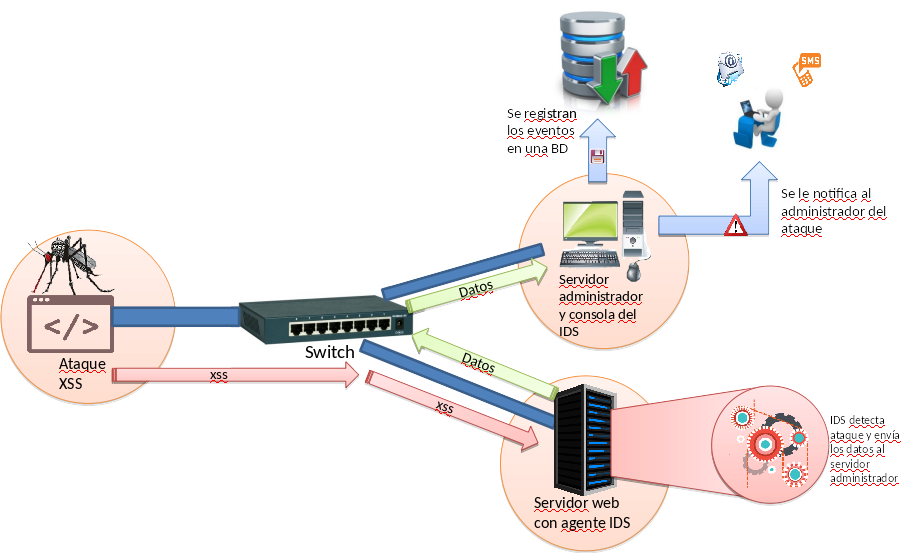
\includegraphics[scale=.6]{images/arquitectura_IDS}
	\caption{Esquema de la arquitectura a implementar.}
	\label{fig:arqui_IDS}
\end{figure}


El ataque XSS será ejecutado sobre una página web vulnerable. Al llegar el ataque al servidor, el tráfico generado por este será analizado dentro del mismo por el agente.\\

Al ser detectado el ataque, el agente envía los datos del ataque al servidor administrador.\\

El servidor administrador registra el evento en una base de datos y envía las notificaciones del ataque. La primera notificación será en la interfaz de monitoreo del sistema y la otra notificación se enviará a las cuentas configuradas de SMS y correo electrónico del administrador encargado.\\

El evento será almacenado en una base de datos para su posterior análisis por el administrador encargado.\\

El administrador recibirá las notificaciones correspondientes por parte del sistema con la información necesaria del evento.\\

El administrador una vez notificado, podrá ver los registros de los eventos ocurridos para tomar las medidas necesarias a la seguridad de sus aplicaciones web.\\

%A futuro se espera que el sistema pueda ser escalable haciendo un sistema más robusto para la detección de ataques XSS e inclusive se pueda agregar módulos para una mayor cobertura de ataques.
